\chapter{基于多尺度密集连接和局部混合注意力的运动想象分类网络}

论文前两个章节主要对运动想象脑电图分类领域的基础知识以及相关研究做了一定的介绍,并且对该领域仍然存在的问题进行了分析。本章对这些问题进行进一步的探讨,针对这些问题提出了一种端到端的新模型DIS-Net:首先,在Inception模型的基础上引入密集连接,构建多尺度密集连接模块,在进行多尺度特征提取的同时,对EEG信号的浅层特征和高级语义信息加以利用,以更完整地获取EEG信号的特征;其次,在以上结构的基础上,针对EEG信号的特性构建了svSE混合注意力模块,将方差信息和时空轴向分离注意力引入注意力计算中,提高模型对EEG信号中的重要特征的关注度。

\section{基于多尺度密集连接和局部混合注意力的分类网络DIS-Net}

DIS-Net的结构如图所示。其分别通过时间卷积层和空间卷积层提取特征,并且都采用了轴向卷积,时间卷积核的大小基于采样频率确定,空间卷积核的大小则基于通道数量确定。此外,由于EEG信号在时间域蕴含更为丰富的信息,并且为了降低对高空间分辨率的依赖,DIS-Net采用集中关注时间维特征的策略,采用更复杂的结构提取时间特征。DIS-Net通过多尺度密集连接模块进行并行特征提取,同时兼顾高级语义信息和低级特征,通过svSE混合注意力模块提升对EEG信号中重要特征的关注度,其结构如图~\ref{fig:dis}~所示。

\begin{figure}[ht]
  \centering
  \includegraphics[width=0.9\textwidth]{dis中2.pdf}
  \caption{DIS-Net结构}
  \label{fig:dis}
\end{figure}

DIS-Net首先通过反转瓶颈层扩展深度,并在深度维度促进时空特征融合。其二通过两个多尺度密集连接模块提取时间特征,在多尺度密集连接模块中,根据EEG信号的采样频率设定每个分支的卷积核大小,从而提取不同尺度的时间/频率特征,并在深度维度对浅层特征和深层特征加以融合。其三,DIS-Net在时间卷积层与空间卷积层之后增加了混合注意力svSE模块,双重校准模型对特征的关注度,减少冗余信息和噪声的MI-EEG分类精度的干扰。其四,DIS-Net通过空间卷积层提取空间特征,且采用了空间轴向卷积和深度可分离卷积。最后,DIS-Net在经过池化、展平、Softmax等操作后,输出预测结果。

在后文中,将依次对DIS-Net的搭建思路和过程进行介绍。

\section{基础网络结构}

卷积神经网络具有强大的特征提取能力,在计算机视觉等领域应用广泛。EEG信号在时间域上具有局部相关性,即相近的时间窗内的信号往往携带相似的信息;在空间域上,EEG信号的局部相关性则较弱,这是因为尽管在采样中,相邻的电极点携带相似的信息,但在数据矩阵中,相邻的电极点未必排列为相邻的行。尽管如此,仍然可以在对网络结构进行针对性调整的情况下,将EEG信号视为二维图像,使用卷积神经网络提取其局部特征。

ShallowConvNet\cite{schirrmeister2017deep}是一个专为端到端解码脑电图信号而设计的深度学习架构,其构思源自EEG信号解码研究领域中广泛使用的FBCSP特征提取算法。ShallowConvNet具有FBCSP算法对频带功率特征高效提取的特性,在实验中证明了能够学习频带功率变化的时间结构特性\cite{schirrmeister2017deep},研究发现,该特性有助于提高分类性能\cite{sakhavi2015parallel}。实验证明,ShallowConvNet在MI-EEG分类领域具有优良的性能\cite{lawhern2018eegnet},其采用四步流程对原始二维输入数据进行处理。具体而言,ShallowConvNet首先通过时间卷积层捕获信号的时间域特征,再通过空间卷积层捕获这些时间特征在不同通道间的空间关联性,随后通过平均池化层进行下采样,最后通过全连接层将多维特征映射至分类输出空间。ShallowConvNet提出的时间卷积与空间卷积相分离的策略是由于EEG原始输入的时域与空域之间的相关性较低,后续的研究大多沿袭了这种方法,论文同样遵循这一思路对EEG信号进行处理。

将EEG原始输入视为具有空间信息的图像数据,论文参考以下几种计算机视觉领域的经典模型,用于网络的特征提取基础结构:

Inception模块起源于经典的GoogLeNet模型\cite{szegedy2015going},并在计算机视觉图像分类任务中取得了优异的效果。传统卷积神经网络倾向于通过加深和拓宽网络结构以增进性能,然而这种做法伴随着参数数量的激增,不仅加大了计算负担,还可能导致过拟合问题。在这种背景下,Inception模块提出了多尺度特征并行提取的策略,旨在保持网络稀疏性的同时,充分利用密集矩阵运算的高性能。典型的Inception-V1模块将不同大小的卷积层和最大池化层并行排列,并行地对输入数据执行多种卷积和池化运算,继而将提取到的不同尺度特征在深度维度上进行拼接。这种设计能够在单层网络内并行地提取输入数据在不同层次和粒度的特征信息,从而在高效扩展网络的深度和宽度的同时,有效削减参数规模,提升计算速度。此外,Inception模块中引入了\(1\times1\)卷积核,用以实现深度上的特征转化和降维,这种方式能够让模型学习到更为丰富的特征,同时降低计算成本。后续的论文中,Inception模块不断迭代优化,陆续引入了批归一化、深度可分离卷积、矩阵因子分解等技术,进一步提升了模型的性能\cite{szegedy2016rethinking,szegedy2017inception}。

残差神经网络是计算机视觉图像识别领域的一个经典模型。ResNet研究发现了深度神经网络的退化现象(Degradation),即随着网络深度不断增加,模型准确率起初随深度上升,却在达到峰值后急剧下滑。针对这种现象,ResNet提出了残差学习框架,其核心思想是引入残差块(Residual Block),每个残差块通过快捷连接(Shortcut Connection)将输入信息直接输送至输出层,使得网络只需要专注学习输入与输出之间的残差信息,而非完整的映射关系。基础的ResNet由一系列残差块堆叠而成,通过快捷连接,ResNet在训练过程中,梯度能够从深层网络直接回传至浅层,避免网络深度增加带来的训练困难和性能下降问题,从而提升深度神经网络的性能表现和训练效率。

U-Net\cite{ronneberger2015u}最初是为生物医学图像分割任务而设计,其具有优秀的性能,尤其在细胞、器官和病变区域的精确标注上表现出色,是医学图像分割领域的主流模型之一。U-Net的独特之处在于其采用了对称的编码-解码结构(Encoder-Decoder)和跳跃连接(Skip Connection)。编码器通过连续的卷积和下采样层对输入图像进行深度特征提取和空间压缩,提炼出高级抽象特征;解码器部分则通过上采样和卷积恢复到与输入图像相同的空间分辨率,同时保留详细的定位信息。跳跃连接将编码器各阶段的特征图直接传递给相应的解码器阶段,有效地结合了包含更多细节信息的浅层特征和包含更多高级语义信息的深层特征,从而在图像分割任务中能够取得更为精细的分割效果。同时,U-Net模型结构简单,易于训练,能够缓解小样本数据集上的过拟合问题。

在这三种模型中,Inception和ResNet均在图像分类任务中展现出了优秀的性能。Inception通过同一层网络内的多尺度特征并行抽取,在不显著增加网络深度的前提下,实现了特征提取的广度与效率的提升。ResNet通过引入快捷连接,解决了深度神经网络训练过程中的梯度消失和退化问题,增强了深层次网络的训练效率和性能表现。U-Net则在生物医学图像分割领域取得了优秀的表现,医学图像的语义信息较为简单,且结构较为固定,因此高级语义信息和低级特征都相对重要,U-Net通过跳跃连接保留并融合了这两类信息,同时,U-Net参数量较小,不容易在小样本数据集上发生过拟合现象。论文选择将U-Net迁移至MI-EEG分类任务中,是因为EEG信号具有与生物医学图像类似的生理特性,如特征相对简单、数据集规模偏小等。

论文通过实验,发现相同的层级设置下,Inception模型具有明显的优势,这可能是出于两方面的原因:其一,过往的研究发现,浅层网络在MI-EEG分类任务上具有良好的表现;其二,EEG信号是由多种频带复合而成的复杂数据,不同大小的卷积核能够提取到不同频率的特征,Inception模块通过多尺度并行的设计,能够提取到多个频率的特征。此外,U-Net模型同样展现出一定的效果,这可能是由于EEG信号具有相对简单的特征,而U-Net通过跳跃连接同时利用浅层特征和高级特征,能够较为完整地利用EEG信号蕴含的信息。

由此,论文选用Inception模块作为MI-EEG信号特征提取的基础结构,旨在保持模型简洁高效的同时,在MI-EEG分类任务中取得更好的性能。

EEG信号的空间分辨率较为不稳定,例如,在BCI Competition IV Dataset 2B数据集\cite{tangermann2012review}中,仅仅使用了三个电极采集MI-EEG信号,使得空间信息相对时间信息更为稀疏。为了减少对高空间分辨率的依赖,论文采取集中关注时间特征的策略,即将Inception模块应用于时间卷积层中,使得时间卷积层的复杂度高于空间卷积层的复杂度,从而保持相对均衡的特征提取。

文献\cite{schirrmeister2017deep,lawhern2018eegnet}指出,在EEG信号解码任务中,增加神经网络的深度有利于提升解码精度。瓶颈层(Bottleneck Layer)是深度神经网络中的常见结构\cite{he2016deep,huang2017densely},通常用于对数据的降维和升维,由于采用了\(1\times1\)卷积进行操作,瓶颈层能够有效地减少神经网络的参数。不同于原始Inception模块中通过瓶颈层进行数据降维的操作,论文使用瓶颈层对数据进行升维操作,并将瓶颈层提取至卷积和池化操作之前,其目标为在深度维度上促进时空信息的融合。此外,论文在模型中引入了批量归一化层和Dropout层,用以加快网络训练速度,并避免小数据集下过早的过拟合。

论文将改进后得到的基础模型称为BaseNet,其结构如图~\ref{fig:BaseNet}~所示。
\begin{figure}[ht]
    \centering
    \includegraphics[width=0.9\textwidth]{Base-Net中2.pdf}
    \caption{BaseNet结构}
    \label{fig:BaseNet}
\end{figure}

\section{基于多尺度密集连接的分类网络}

在构建BaseNet时,论文发现U-Net在处理MI-EEG分类任务时同样展现了一定的优势。由于EEG信号的特征相对简单,因此低级特征与高级语义信息都相对重要,U-Net因其特殊的跳跃连接结构有效地融合了这两种信息,然而,U-Net中通过解码器阶段将特征图恢复至原始空间尺寸的操作并非必要,因为在分类任务中,这种重建过程可能导致额外的计算负担且对分类性能的提升效果不明显。因此,论文从U-Net兼顾低级特征与高级语义信息的策略中得到启发,同时对不必要的特征图空间尺寸还原过程进行规避,以构建一个既能充分利用EEG信号中各级别特征信息,又具备高效计算能力的改进模型。

\subsection{多尺度密集连接}

Gao Huang等人提出了密集连接网络(Dense Convolutional Network,DenseNet)\cite{huang2017densely}。在ResNet的基础上,DenseNet提出了一种更为激进的连接模式:引入从任意层到后续层的直接连接,即密集连接(Dense Connection)。DenseNet的第 \(l\) 层接收所有前序特征图为输入,其输出为 \(x_l\),计算如公式~\ref{eq:dense-conn}~所示。
\begin{equation}
  x_l = H_l([x_0, x_1, ···, x_{l-1}])
  \label{eq:dense-conn}
\end{equation}
其中,\([x_0, x_1, ···, x_{l-1}]\) 代表第 \(0, ···, l-1\) 层的输出特征图,\(H_l(·)\) 代表非线性转换复合函数,可能包括一系列的批量归一化、ReLU、池化及卷积操作。密集连接的结构如图~\ref{fig:denseBlock}~所示。
\begin{figure}[ht]
  \centering
  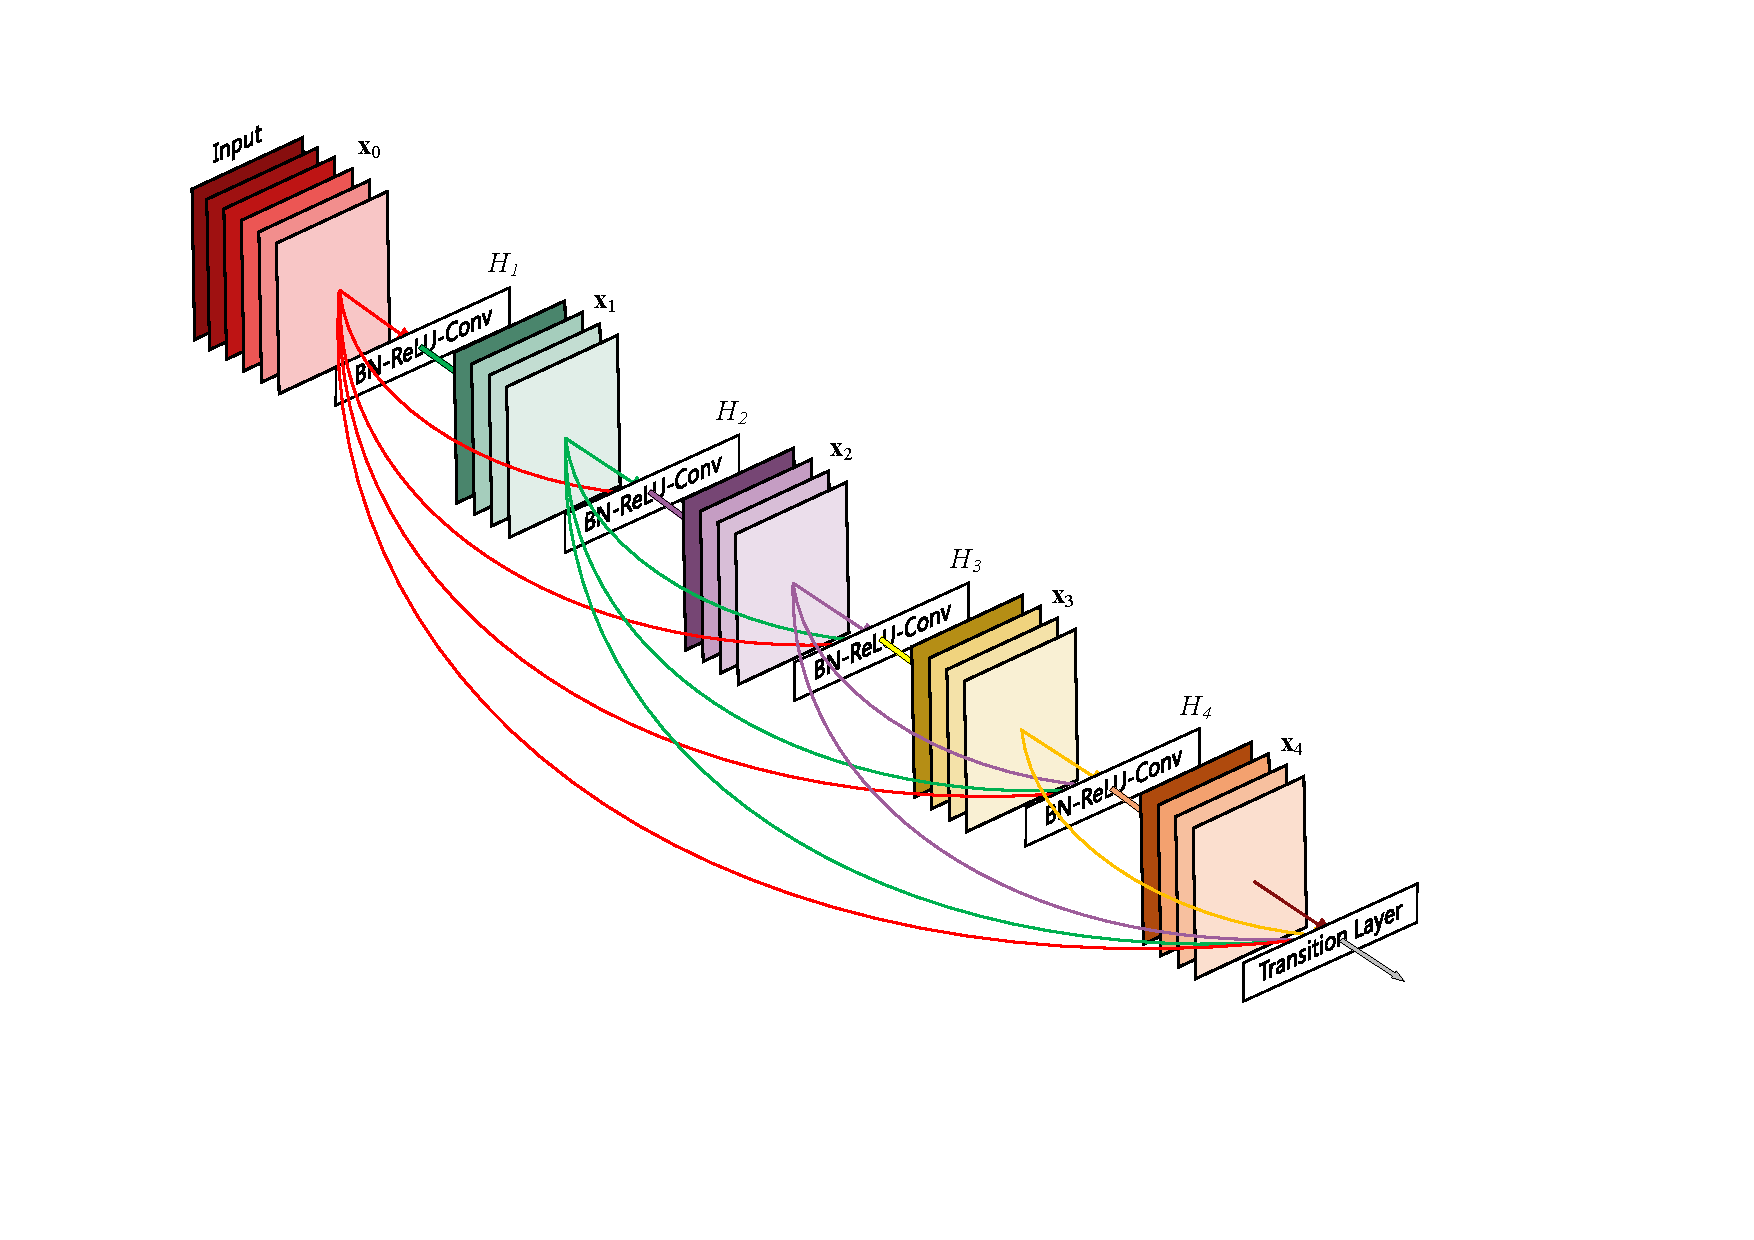
\includegraphics[width=0.5\textwidth]{denseBlock.pdf}
  \caption{密集连接结构\cite{huang2017densely}}
  \label{fig:denseBlock}
\end{figure}

在密集连接模块中,所有的前序特征图通过Concentrate在深度维度上连接在一起,因此,在一个密集连接模块中所有特征图的大小是相同的。DenseNet提出了Transition模块用于连接两个相邻的密集连接模块,并通过池化操作对特征图进行下采样,从而减小特征图的大小。

通过密集连接的方式,网络中的每一层都能够访问并整合所有前序层提取出的特征信息,进而充分利用EEG信号中的低层特征细节和高层语义信息。相较于U-Net中的编码-解码结构,密集连接无需经历数据空间的重建过程,即可实现特征的有效复用。此外,DenseNet中的Transition模块也为实现特征图的下采样提供了思路。

为了同时利用Inception模块多尺度并行特征提取和密集连接兼顾深层与浅层特征的优点,论文选择将DenseNet嵌入Inception模块中,替代原本的时间卷积核,称之为多尺度密集连接模块(Dense Inception Module)。

原始的密集连接模块在计算机视觉图像分类任务中都取得了优秀的表现,在设计上,它考虑到了图像数据在空间维度上的局部相关性,然而,EEG信号的时空域局部相关性较低,需要对原始密集连接模块的卷积核进行改造。研究指出\cite{lawhern2018eegnet},当设计用于提取EEG特征的卷积核时,将时间卷积核长度设置为EEG信号采样率的一半,可以有效地捕获2Hz及以上频段的信号信息。因此,在处理EEG信号时,时间卷积核的长度应当依据EEG信号的实际采样率来灵活设定,以便提取不同频率成分的信号特征。

将密集连接模块中的卷积核概念转化为针对时间序列的一维卷积(尽管在实现时仍采用二维卷积),为了更好地匹配EEG信号的采样特性及其内在频率成分,依据EEG信号的采样频率 \(sfreq\) 来动态调整位于Inception第 \(i\) 个分支上的密集连接模块的时间卷积核大小 \(kernel_i\),具体如公式~\ref{eq:kernel_cal}~所示。
\begin{equation}
    kernel_i = \left \lfloor \frac{sfreq}{2 \times i} \right \rfloor , \quad i \in (1,2,...,5)
    \label{eq:kernel_cal}
\end{equation}
其中,\(sfreq\) 是EEG信号的采样频率。这样设置卷积核大小是为了更全面地捕捉EEG信号中不同频率成分的特征信息,同时避免因卷积核大小过于接近而导致提取的特征之间重叠度过高。例如,当\(i=1\)时,卷积核大小将是采样率的一半,进而能够有效地捕获到2Hz及更高频段的EEG信号特征。

由此,第\(i\)个分支上的密集连接模块的非线性转换复合函数 \(H(·)\) 包含的步骤如图~\ref{fig:dense-kernel}所示。
\begin{figure}[ht]
    \centering
    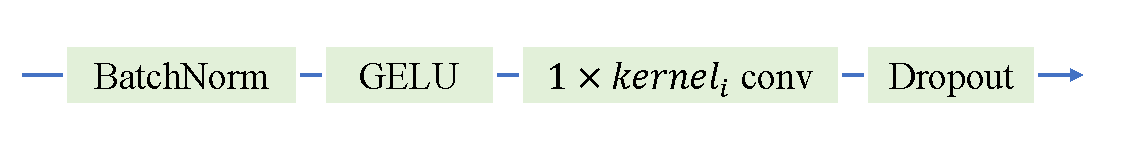
\includegraphics[width=0.7\textwidth]{密集连接模块.pdf}
    \caption{非线性符合转换函数}
    \label{fig:dense-kernel}
\end{figure}

\subsection{基于多尺度密集连接的分类网络DI-Net}

将多尺度密集连接模块融入基础网络模型BaseNet中,构建出新模型DI-Net,其结构如图~\ref{fig:incep-dense}~所示。在BaseNet的基础上,由Dense Inception Module构成时间卷积层,其内部的各个分支均由一系列改进版的Dense Block紧密堆叠而成,形成密集连接结构,用以同时获取浅层和深层的时间特征。对于每个Dense Block,论文依据EEG信号的特性,对其非线性转换函数进行了改进,从而在MI-EEG分类任务上取得更好的效果。每个分支提取的特征图在深度维度上进行聚合,并通过Transition模块进行深度压缩和特征整合,以进一步提升模型的表达能力和计算效率。
\begin{figure}[ht]
  \centering
  \includegraphics[width=0.9\textwidth]{incep-dense中2.pdf}
  \caption{DI-Net结构}
  \label{fig:incep-dense}
\end{figure}

\section{结合局部注意力的分类网络}

根据神经科学先验知识,EEG信号中不同的通道和采样点具有不同的重要性,这为在MI-EEG分类领域应用注意力机制提供了理论依据。论文选择将注意力注意力机制引入模型中,以提高模型对EEG信号重要特征的关注度。

\subsection{局部混合注意力svSE}

将二维EEG信号视为一种由通道和时间两个维度构成的特殊图像,使得在MI-EEG分类领域能够迁移应用计算机视觉领域中的注意力机制。计算机视觉领域中经常使用的注意力机制有通道注意力、空间注意力、混合注意力机制等。
    
不同于EEG信号中代表电极的通道,计算机视觉领域的通道代表图像的不同特征映射。通道注意力机制用于调整不同特征通道的重要性,通常会对每一个特征通道计算一些全局统计量,如均值、方差等,再将这些统计量经过非线性变换层进行编码,最后将编码向量进行转换并用于各个特征通道的加权。通道注意力机制的经典模型是压缩和激励网络(Squeeze-and-Excitation Networks,SENet)\cite{8578843},其主要思想即是压缩(Squeeze)和激励(Excitation),SENet首先通过压缩操作获取全局上下文信息,然后通过激励操作对每个通道独立生成权重系数。具体而言,在压缩操作中,SENet在空间维度执行全局池化操作,将每个通道的特征图汇总成一个标量值;然后,在激励操作中,SENet通过一个全连接网络生成每个通道的权重系数,这些权重系数用于重新加权每个通道的特征图,以增强有用的特征并抑制无用的特征。

在后文中,为避免与计算机视觉领域中的概念相混淆,在MI-EEG分类任务中,用深度来代表EEG信号的不同特征映射,而通道仍然代表电极。
    
在计算机视觉领域中,空间注意力机制用于调整图片、视频等输入数据在空间维度中不同区域的重要性,通常会在深度维度上通过全局池化、卷积、特征融合等操作生成一个与特征图尺寸相同的注意力图,其值反映了空间维度中不同区域的注意力强度,最后,将注意力图进行转换,并用于原始特征图的加权。空间注意力机制的经典模型是空间变换网络(Spatial Transformer Network,STN)\cite{jaderberg2015spatial},其具有对输入数据进行空间变换的能力,能够自动捕获重要区域的特征。
    
混合注意力机制是一种集成多种注意力机制的方法,旨在更全面地捕获和整合输入数据在不同维度的有效信息。混合注意力机制通常会使用不同的注意力机制分别计算原始特征图的注意力权重,再将这些注意力权重进行融合,最后将融合后的注意力权重用于原始特征图的加权,或者将不同的注意力权重用于原始特征图加权,再将加权特征图进行融合。混合注意力机制的经典模型有卷积注意力机制模块(Convolutional Block Attention Module,CBAM)\cite{woo2018cbam}、空间与通道压缩与激励模块(Spatial and Channel Squeeze-and-Excitation,scSE)\cite{roy2018concurrent}等。
    
CBAM结合了通道注意力机制与空间注意力机制,输入特征图首先经过通道注意力模块进行加权,再通过空间注意力模块进行加权,从而得到最终结果。

具体而言,在通道注意力模块中,输入特征图分别进行空间维度上的全局最大池化和全局平均池化,再将得到的统计值分别通过一个共享权重的全连接层,最后经过逐点加和与非线性变换得到通道注意力权重,用于输入特征图的加权。空间注意力模块的输入是经过通道注意力加权的特征图,首先在通道维度上进行全局最大池化和平均池化,再将得到的统计值在通道维度进行拼接,最后经过卷积降维与非线性变换得到空间注意力权重,与特征图加权后得到最终结果。

scSE同样结合了通道注意力机制与空间注意力机制,基于SENet提出了一种通道注意力模块(Channel Squeeze-and-Excitation,cSE)和一种空间注意力模块(Spatial Squeeze-and-Excitation,sSE),不同于CBAM,scSE的两个子模块并行处理原始输入,分别在空间维度和通道维度对原始输入进行加权,最后再进行特征图的融合。具体而言,cSE模块中,原始输入依次经过了空间维度的全局平均池化,通道维度的卷积降维与升维,以及非线性变换,以得到通道注意力权重。sSE模块中,直接通过深度卷积在通道维度进行降维,再经过非线性变换以得到空间注意力权重。

注意力机制通过动态分配权重,使得模型能够聚焦于输入数据中的关键信息,削弱噪声的影响,混合注意力机制则结合了多种注意力机制的优点,从而能够更全面地捕获和整合不同维度的数据特征,并在许多情况下展现出优于单一注意力机制的性能。因此,论文将升维处理后的EEG信号视作具有深度信息的图像数据,采用结合了深度注意力和空间注意力的混合注意力机制对DI-Net进行改进。

CBAM模块和scSE模块均为轻量级注意力模块,且均兼顾深度注意力和空间注意力,但实验发现scSE模块在MI-EEG任务上具有更好的表现。与此同时,文献\cite{roy2018concurrent}研究发现scSE模块在语义分割任务上表现出色,特别是在与EEG信号拥有相似生理特性的医学图像的分割任务,其性能优于CBAM模块。基于以上理由,论文选择基于scSE模块进行改进,提出了一种新的注意力机制svSE(Separate Variance-Informed Spatial and Channel Squeeze-and-Excitation)模块,其结构如图~\ref{fig:svSE}~所示。
\begin{figure}[ht]
    \centering
    \includegraphics[width=0.9\textwidth]{svSE中2.pdf}
    \caption{svSE结构}
    \label{fig:svSE}
\end{figure}

针对cSE模块,采用全局最大池化取代全局平均池化操作,用以突出显著特征,得到权重图\(Att_c \in \mathbb{R}^{D \times 1 \times 1}\)。针对sSE模块,论文提出两种方式进行改进,并将两种方式所得的权重相结合以获取最终的输出:

(1) 由CBAM模块的多维全局池化思想以及FBCNet模型的方差层设计\cite{mane2021fbcnet}得到启发,对于输入\(X \in \mathbb{R}^{D \times C \times T}\),采用深度维度上的全局平均池化和全局方差计算操作代替原模块中的压缩操作,得到\(X_{pool} \in \mathbb{R}^{2 \times C \times T}\),随后通过\(1\times1\)卷积对特征图在深度维度进行聚合,得到的权重图\(Att_v \in \mathbb{R}^{1 \times C \times T}\),更好地表征EEG信号的时序变化特性;

(2) 考虑EEG信号中的时空权重低相关性,即空间特征权重代表电极重要程度,时间特征权重代表采样点重要程度,分两个维度提取特征,获取轴向注意力。对于输入\(X \in \mathbb{R}^{D \times C \times T}\),在空间维度,首先使用\(1\times1\)卷积进行深度压缩操作获得\(X_{sf} \in \mathbb{R}^{1 \times C \times T}\),随后通过时间维度上的平均池化和最大池化得到两个特征图,获得\(X_{spool} \in \mathbb{R}^{2 \times C \times 1}\),通过\(1\times1\)卷积对这两个特征图进行融合,得到\(X_s \in \mathbb{R}^{1 \times C \times 1}\)。对于时间维度,进行空间维度上的卷积操作,以得到时序权重\(X_t \in \mathbb{R}^{1 \times 1 \times T}\)。最后,将空间权重与时序权重以克罗内克积(Kronecker)的方式相乘,恢复维度,得到最终的权重图\(Att_s \in \mathbb{R}^{1 \times C \times T}\)。

其中,\(D\)为输入的深度,\(C\)为空间(通道),\(T\)为时间。此外,使用Softmax激活函数替换Sigmoid激活函数,旨在更好地利用全局信息。由此,整个svSE模块的公式如公式~\ref{eq:svse}~所示。
\begin{equation}\label{eq:svse}
    \begin{aligned}
        &Att_{vs}=Att_v \oplus Att_s \\
        &X_1=Expand(Att_{vs}) \odot X \\
        &X_2=Expand(Att_c) \odot X \\
        &X_{svSE}=X_1 \oplus X_2
    \end{aligned}
\end{equation}
其中,\(\oplus\)为逐元素相加,\(\odot\)为逐元素相乘,\(X_{svSE}\)为加权后的输出。

\subsection{分类网络结合svSE模块}

svSE是一个即插即用的、特定于MI-EEG分类任务的注意力模块,其通过引入方差信息,更好地对EEG信号的时变特征进行表征,通过轴向时空注意力对EEG信号的低局部时空相关度加以适应,在减少了计算开销的同时对重要特征加以关注,适应不同的数据分布。

在DI-Net的基础上,svSE模块有三种方式加入模型,分别是在时间卷积层之后加入、在空间卷积层之后加入,以及在时空卷积层之后都加入。根据实验结果,第三种方式能够取得最好的性能表现,且由于svSE模块是轻量级注意力模块,此种方式相较于其他两种方式仅仅增加了少量参数,因此,论文选择第三种方式将svSE模块引入DI-Net中,即将svSE模块同时加入DI-Net的时间卷积层与空间卷积层之后。由此,得到了本章提出的模型DIS-Net,其结构如图~\ref{fig:dis}~所示。

\section{本章小结}

本章主要对论文基于多尺度密集连接和混合注意力所提出的模型进行了详细的介绍,对一系列改进点进行了详细的阐述,并最终构建出一种端到端的运动想象分类网络DIS-Net。首先,论文针对EEG信号的时频空特性,基于Inception和反转瓶颈层提出了基础网络BaseNet,并调整了BaseNet的卷积层分布与卷积核大小,从而实现时空特征的融合和特定频段特征的提取。其次,论文针对EEG信号特征相对简单的特性,构建了多尺度密集连接模块,将密集连接机制引入Inception模块之中,从而在增加特征提取的深度和广度的同时,对浅层和深层特征加以融合利用。最后,论文针对EEG信号信噪比低且非平稳的特性,提出了引入方差池化与轴向时空注意力的混合注意力模块svSE,对重要数据进行关注,从而增强模型对伪迹噪声的抗噪性能,以及对不同分布的数据的处理能力。

